\chapter{CPU设计方案}

\cpuname 采用对称双发射顺序执行,共有5级流水。\cpuname 的数据通路示意图如\ref{img:datapath}所示,其中红线部分为master path,蓝线部分为slave path。在对称双发射中,master和slave的主要区别在于前者先于后者执行,在处理异常、提交等事宜时会被优先处理。当然,上述的“对称”双发射,只是相对于只支持ALU指令双发的非对称逻辑而言,\cpuname 的设计中slave path支持的功能和master path旗鼓相当。但严格来讲,并不是绝对对称,在处理跳转指令、例外指令、写TLB指令等这类可能刷新流水线的指令时,需要优先在master处理,这在后续的双发策略中会详细说明。

% \begin{landscape} % 用于旋转页面
\begin{figure}[h]
    \centering
    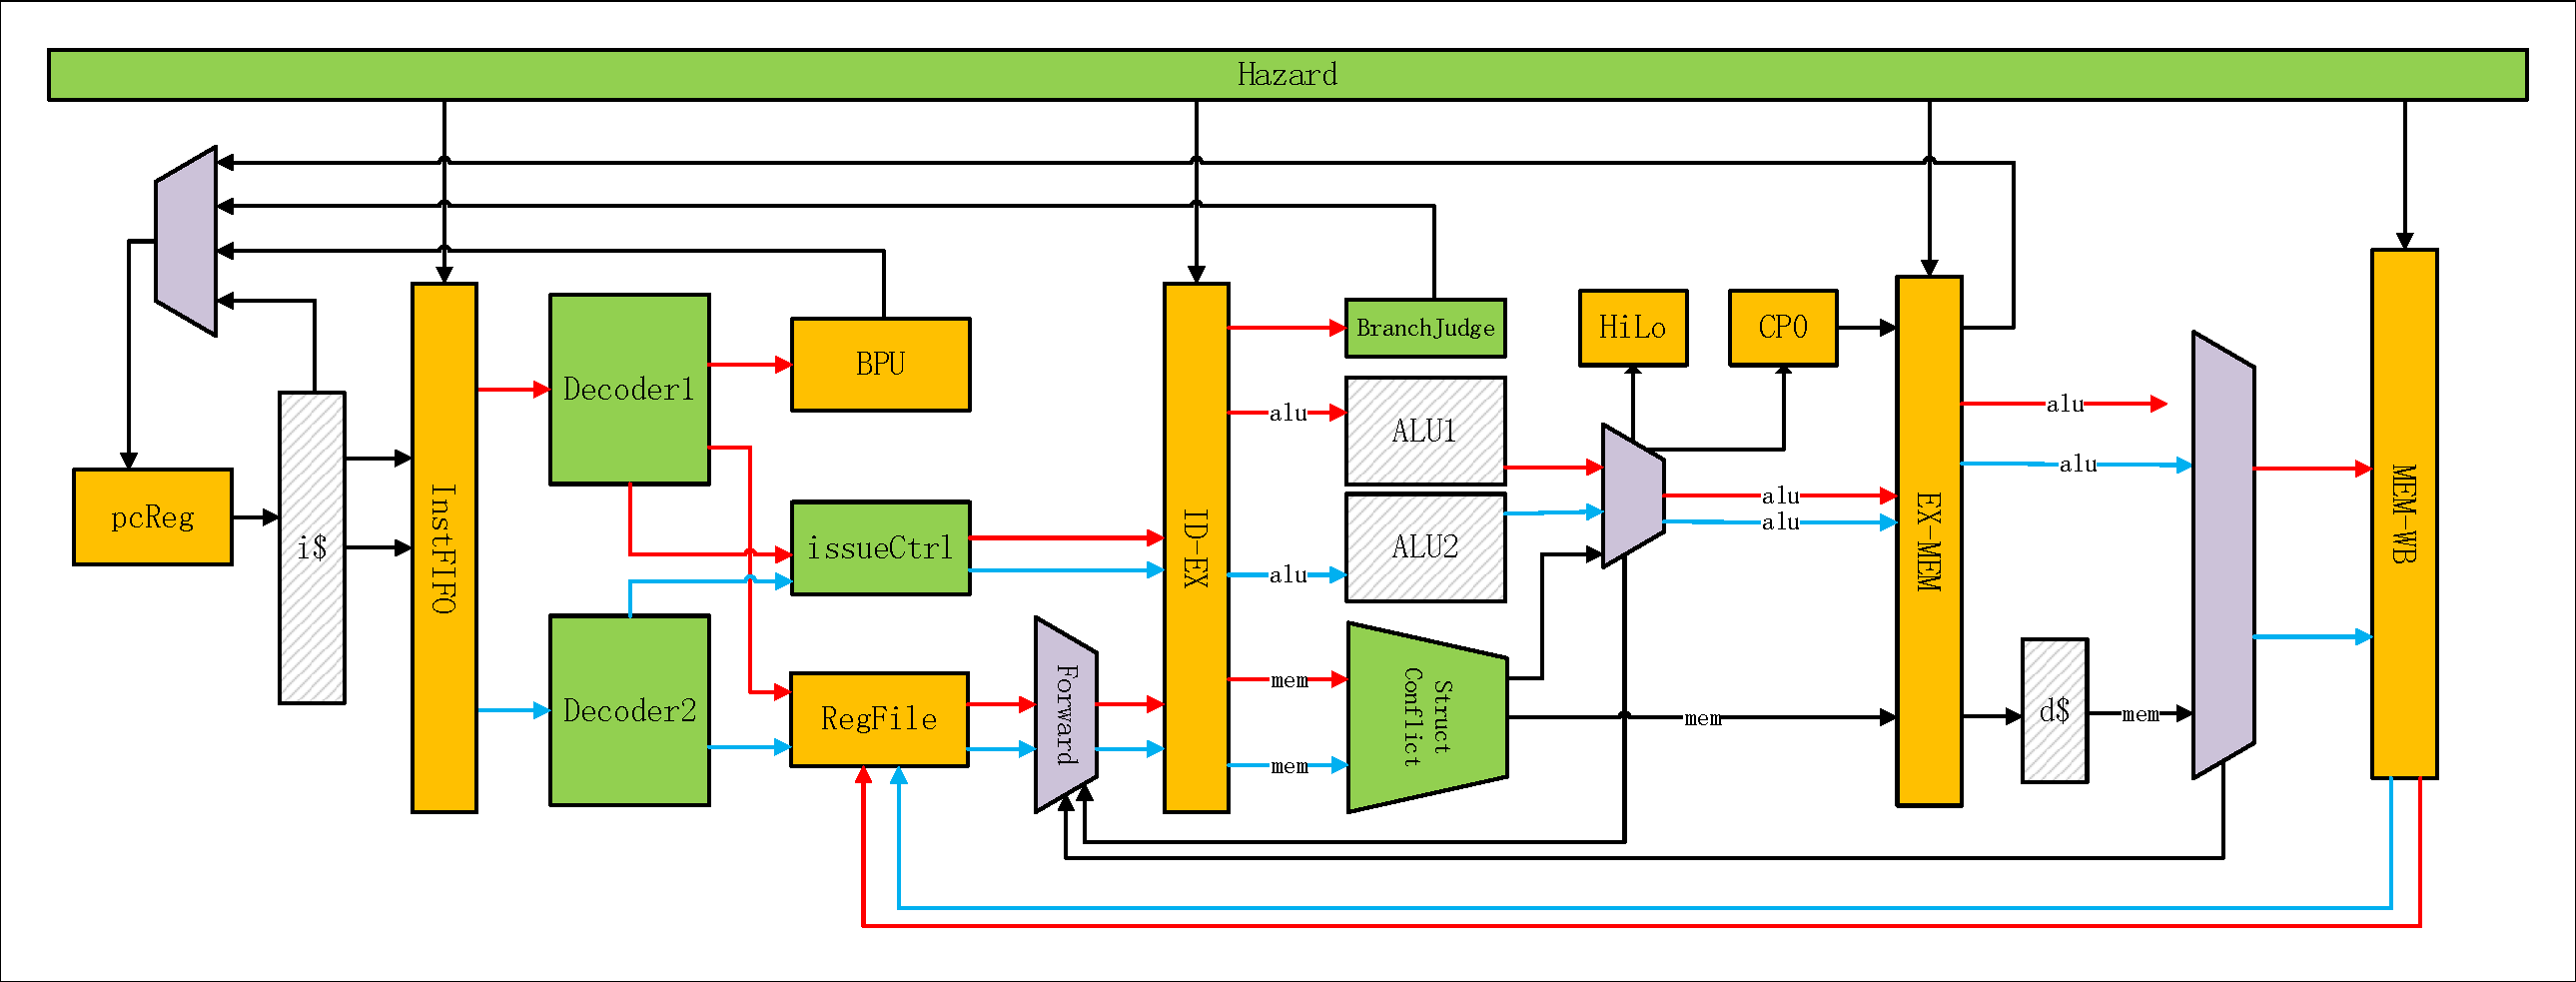
\includegraphics[width=\linewidth]{datapath.pdf}
    \caption{数据通路设计图}
    \label{img:datapath}
\end{figure}
% \end{landscape}


\section{双发策略}
在双发射的CPU设计中,双发策略会影响整个数据通路的设计,故我们先来介绍一下\cpuname 的双发策略,即分情况讨论slave是否发射。其中在提供的代码中,issueCtrl模块解释了\cpuname 的整个双发策略。

\begin{enumerate}
    \item \textbf{only\_master类指令}: 即只能放在master发射,且slave不发射指令。对于可能触发例外的指令(如MTC0、SYSCALL、ERET、BREAK、TLBWI等指令),会导致PC跳转到异常处理地址或其返回地址处,进而刷新整个流水线。对于这类指令,如果在slave中检测到这类指令,则暂停slave发射,将其延迟到下一周期的master发射;如果在master中检测到这类指令,也会暂停slave发射,避免不必要的流水线刷新。
    \item \textbf{only\_in\_master类指令}: 即只能放在master发射,且slave可发射指令。 对于跳转指令,在一定条件下会跳转到其他地址,并刷新整个流水线。和only\_master不同的是,跳转指令会涉及到延迟槽的处理。故如果在slave中检测到这类指令,则暂停slave发射,将其延迟到下一周期的master发射;如果在master中检测到这类指令,若满足slave发射条件,则发射该条指令(延迟槽),若不满足,则在下一周期的master中发射延迟槽数据。
    \item \textbf{数据冲突}
    \begin{enumerate}
        \item \textbf{RAW冲突}:检查master和slave之间是否存在HiLo、CP0、GPR等寄存器的RAW情况,若存在,则slave不发射。
        \item \textbf{Load To Use 冲突}:检查slave读到的寄存器是否是当前在E阶段执行的读存指令的结果,若是,则slave不发射。
    \end{enumerate}
    \item \textbf{结构冲突}:由于设计的乘除单元、访存单元只有一个,故二者会产生结构冲突。若master和slave同时需要占用这类单元,则slave不发射。
    \item \textbf{数据有效性}:slave发射的前提是master必须要发射或当前第二条指令有效。若遇到master暂停发射或指令FIFO为空的情况下,slave不发射。
\end{enumerate}


\section{数据通路设计}
\subsection{取指阶段}
为了保证双发射能够正常执行,第一要素便是“一次取指能够取回多条指令”,才能保证传到D时,至少有两条指令可以准备用于双发射。指令Cache一行64bit的设计,也正适应了双发逻辑中取指的特点,使得\cpuname 传入指令Cache一个PC地址,可获得该PC及PC+4对应的两条指令。值得注意的是,为了简化Cache命中逻辑(即不存在跨Cache Line访问Cache的情况),传回数据中,并不是所有PC都会传回2条指令,故我们添加了inst\_data\_ok信号表示取回的指令是否有效。\cpuname 的设计中,一行共2字,如果PC索引到该行的最后一个字,Cache只传回1条指令,inst\_data\_ok2置为0;除此之外,传回两条数据,inst\_data\_ok1和inst\_data\_ok2均置为1。

出于双发策略中,slave并不是每次都会发射,故取回的数据需要缓存下来,以用于下次使用,节省Cache访问时间。\cpuname 中,使用指令FIFO,将传回的有效指令缓存下来。使用指令FIFO还有一个好处是可以分割取指和后续阶段,即取指不受后续阶段产生的阻塞影响(但为了保证结果的正确执行并简化控制逻辑,后续阶段仍然会受到指令Cache产生的stall影响)。其中,如果指令FIFO放满,则暂停前段取指;如果指令FIFO为空,则暂停后续发射。

\subsection{译码阶段}
Instruction Decode阶段中,主要完成以下操作:
\begin{itemize}
    \item \textbf{译码}:从FIFO中读出指令,立即进入译码模块。译码模块中,会分析该指令的功能,并分配控制信号。
    \item \textbf{分支预测阶段}:为了减少分支跳转带来的流水线刷新数量,我们添加了静态分支预测单元,利用pc低位记录跳转数据,利用传统2bit策略更新跳转数据的记录。在D阶段获取到指令后,立即根据该指令所在PC进行预测,其中为了减少译码带来的延迟,分支预测单元内部单独进行分支译码,若是分支指令,即可取出预测结果并更新取指阶段的PC。
    \item \textbf{发射判断}:译码结束后,需要进入issueCtrl模块进行发射判断,发射判断结果会返回到指令FIFO中,控制FIFO的读指针的增量。
    \item \textbf{数据准备}:读取regfile中对应的GPR数据,准备好数据后进入Excute阶段执行(在\cpuname 中,regfile具有4个读端口和2个写端口)。其中为了在执行阶段的开头即可直接使用准确的数据,我们将数据前推单元放在了译码阶段的末尾。值得注意的是,为了减少前推带来的延迟,译码阶段中需要GPR数据的模块,均使用GPR直接读出的数据,而不是前腿数据(如JR类指令目标地址的计算),若此时存在RAW冲突,则需要推迟到执行阶段进行计算。
\end{itemize}

\subsection{执行阶段}
Excute阶段中,主要完成以下操作:
\begin{itemize}
    \item \textbf{跳转处理}:在译码阶段中,Branch指令需要在执行阶段中判断跳转是否成功,并将判断结果送回分支预测单元进行数据更新,更新此时取值阶段的PC并刷新流水线。同理,如果是译码阶段遇到数据冲突的JR类指令,其在本阶段获取到准确的目标地址后,更新此时取值阶段的PC并刷新流水线。
    \item \textbf{ALU计算}:可以处理单周期运算指令和多周期运算指令。其中,多周期运算指令包括乘除法指令。\cpuname 中乘法指令需要2周期、除法指令需要35周期,且在运算完成前会产生stall信号,阻塞D、E、M、W四个阶段。其中,为减少资源占用,流水线中只提供一个乘法器和除法器,故master和slave在使用时需要进行仲裁。同时获取到乘除结果后,即在执行阶段写HiLo寄存器,以期在访存阶段即可获取新的HiLo数据值,避免了HiLo数据的前推。
    \item \textbf{访存仲裁及其地址计算}:由于data cache是BRAM结构,需要一个周期取出数据,我们需要在E阶段将访存信号传递给Data Cache。因为master和slave都支持访存(但不会同时访存),故在传递访存前,需要用StructConflict模块进行仲裁;并保证访存阶段的刷新信号置0且使能信号置为1,以使访存信号能由E阶段正常传到M阶段,保证访存阶段数据的正常传回。同时,为了减少访存地址计算经过的路径,我们分离了执行阶段中的ALU路径和MEM路径(如图 \ref{img:datapath} 所示),单独利用base(rs value) + offset(immediate value)计算访存地址。同时根据访存地址及其比特要求对传给Data Cache的地址进行地址错例外判断(AdEl和AdEs判断。
    \item \textbf{TLB地址转换}:在上一个小点中,能够获取到访存虚拟地址,此时将访问 L1 TLB 进行初步的映射地址翻译,以便于提前访存。
    \item \textbf{异常汇总}:由上述可以看出,在执行阶段,可以获取从任何指令涉及到的所有异常信号,故我们在执行阶段汇总异常信号,并更新CP0寄存器,以期在访存阶段即可获取新的CP0数据值,避免了CP0数据的前推。
\end{itemize}

\subsection{访存阶段}
Memory Access阶段,主要完成以下操作:

\begin{itemize}
    \item \textbf{访存控制}:虽然在E阶段传递给了Data Cache基本的访存信号,告知Data Cache需要准备对应地址的数据;但是并没有告知需要取出的数据的比特数。E阶段汇总时若发现异常,则传到M阶段后,会将Data Cache的握手信号data\_sram\_enM将会置为0,阻止Data Cache将错误的地址传到AXI总线上。反之,则正常发送data\_sram\_enM信号,并得到传回的数据,再通过StructConflict模块,将数据交付到对应path(master或slave)上。
    \item \textbf{写回数据选择}:master和slave两条路径上的计算结果(alu)和访存结果(mem)的选择。
\end{itemize}

\subsection{写回阶段}
Write Back阶段,主要执行写回GPR请求。若此时读取GPR的地址,恰好是写GPR的地址,需要进行写前递操作。

\section{冲突处理}
\subsection{数据冲突}
\begin{itemize}
    \item \textbf{RAW冲突}:当master或slave需要读取的数据是已经发射且进入后续流水阶段的指令,会产生RAW冲突。本设计将需要的数据均前推到D阶段,前推后立即进入触发器,避免前推数据所在关键路径过长。其中,若需要读取的数据是当前E阶段的访存数据,则需要进行阻塞以等待访存数据在M阶段返回。若需要读取的数据是当前E阶段的计算结果、或M阶段的计算结果、或M阶段的访存结果,则通过forward\_top模块前推到D阶段。
    \item \textbf{WAW冲突}:当同周期的master和slave写入寄存器的地址一致时,会产生WAW冲突。因为slave是master后一条指令,故regfile更新时,会优先写入slave的结果。
    \item \textbf{WAR冲突}:由于本设计为顺序流水线,故不存在WAR冲突。
\end{itemize}

\subsection{结构冲突}
当master和slave同时需要访存或占用乘法器或占用除法器时,会产生结构冲突。本设计中,结构冲突的指令只发射master一条,保证CPU正确执行。

\subsection{控制冲突}
当遇到跳转指令时,会产生控制冲突。MIPS指令系统中,跳转指令包含延迟槽。本设计中,若产生跳转(译码阶段或执行阶段),则根据发射情况判断当前fifo中的第一条读数据是否是延迟槽数据。如果是,则需要判断当时是否有阻塞信号,若没有则直接执行该第一条读数据,若有则需要保留该数据到指定delayslot\_data寄存器,以备阻塞取消后使用;此外跳转会引起流水线的刷新,但需要保证延迟槽数据能够不被刷新并正常流入下一阶段执行。如果不是,则正常刷新流水线即可。

\section{CP0寄存器}
在自定义CPU中扮演着小型操作系统角色的CP0,具有异常处理、内存管理、系统控制等功能。
为了支持MIPS指令系统的正常功能运行,我们设计的CP0处理器包含的基本寄存器如表\ref{table:base_cp0}所示。

\begin{table}[!htbp]
    \centering
    \caption{基本的CP0寄存器}
    \label{table:base_cp0}
    \begin{tabular}{ccll}
        \toprule
        \multicolumn{1}{c}{\textbf{编号}} & \multicolumn{1}{c}{\textbf{选择}} & \multicolumn{1}{c}{\textbf{名称}} & \multicolumn{1}{c}{\textbf{功能定义}} \\ 
    \midrule
    8   & 0 & BadVAddr  & 记录最新地址相关例外的出错地址 \\
    9   & 0 & Count     & 处理器内部计数器 \\
    11  & 0 & Compare   & 计时中断控制器 \\
    12  & 0 & Status    & 处理器状态与控制寄存器 \\
    13  & 0 & Cause     & 存放上一次例外原因 \\
    14  & 0 & EPC       & 存放上一次发生例外指令的 PC \\
    15  & 0 & PRId      & 处理器版本和标识符 \\
    15  & 1 & EBase     & 中断向量基地址寄存器 (MIPS Release2必需) \\
    16  & 0 & Config0   & 处理器配置 \\
    30  & 0 & ErrorEPC  & 上一次发生例外的计数器数值 \\
    \bottomrule
    \end{tabular}
\end{table}

在添加TLB时,需要涉及内存管理相关的CP0寄存器,如表\ref{table:mmu_cp0}所示。

\begin{table}[!htbp]
    \centering
    \caption{MMU相关的CP0寄存器}
    \label{table:mmu_cp0}
    \begin{tabular}{ccll}
    \toprule
    \multicolumn{1}{c}{\textbf{编号}} & \multicolumn{1}{c}{\textbf{选择}} & \multicolumn{1}{c}{\textbf{名称}} & \multicolumn{1}{c}{\textbf{功能定义}} \\ 
    \midrule
    0   & 0 & Index     & TLB 数组的索引 \\
    1   & 0 & Random    & 随机数 \\
    2   & 0 & EntryLo0  & TLB 项的低位 \\
    3   & 0 & EntryLo1  & TLB 项的低位 \\
    4   & 0 & Context   & 指向内存中页表入口的指针 \\
    5   & 0 & PageMask  & 控制 TLB 的虚拟页大小 \\
    6   & 0 & Wired     & 控制 TLB 中固定的页数 \\
    10  & 0 & EntryHi   & TLB 项的高位 \\
    28  & even  & TagLo & 缓存标签 Tag 的低位 \\
    29  & even  & TagHi & 缓存标签 Tag 的高位 \\
    \bottomrule
    \end{tabular}
\end{table}

\section{中断和异常}
为使处理器的功能完整,\cpuname 支持异常处理。根据MIPS规范要求,\cpuname 支持精确异常,即出现异常后,准确记录发生异常的指令地址,并存放在EPC寄存器中以待异常返回时使用;且保证发生异常前的所有指令正常提交;发生异常的指令及其之后的指令不提交,并跳转至异常处理程序入口进行异常处理。\cpuname 中支持的指令优先级顺序如下:

\begin{enumerate}
    \item \textbf{中断例外}:包括硬件中断、软件中断和计时器中断。
    \item \textbf{地址转换异常}:访问TLB时,TLB表中没有有效的转换对应项可用时,会发生地址转换异常,包括TLB重填异常、TLB无效异常(有load页无效、store页无效、modify页无效等)等。
    \item \textbf{地址错例外(取指)}:PC地址未对齐四字节。
    \item \textbf{保留指令例外}:当执行一条未实现的指令时,触发保留指令例外。
    \item \textbf{自陷例外、系统调用例外}:执行到Syscall、Break等自陷指令时。
    \item \textbf{整型溢出例外}:执行ADD,SUB,ADDI,SUBI等指令发生溢出时。
    \item \textbf{地址错例外(数据访问)}:访问数据的地址未对齐,包括AdEl、AdEs两类错误。
\end{enumerate}

其中中断例外为异步例外,其他异常例外为同步例外。\cpuname 的设计中,某时刻发生的中断,将被绑定在D阶段执行的指令及其pc上。